%%% B.A.T.M.A.N Experimental (BMX) Reference Manual
%%% Copyright (C) 2007 Axel Neumann <axel (at) open-mesh.net>
%%% Licensed under the Creative Commons BY-NC-SA-2.0
%%% http://creativecommons.org/licenses/by-nc-sa/2.0/


\documentclass[11pt]{article}
%\documentclass[11pt]{report}
\usepackage{fancyheadings}
\usepackage{multicol}
\usepackage{graphicx}
\usepackage[latin1]{inputenc}

\newcommand{\thisdate}{\today}
\newcommand{\thisauthor}{Axel Neumann}
\newcommand{\thistitle}{B.A.T.M.A.N Experimental (BMX) Reference Manual}
%\newcommand{\bsv}{\begin{verbatim}}
%\newcommand{\esv}{\end{verbatim}}

\setlength{\textheight} {21.5cm}
\setlength{\textwidth}  {15.5cm}
\setlength{\oddsidemargin}  {0cm}

\input epsf

\pagestyle{fancyplain}
\setlength{\headrulewidth}{0.4pt}
\setlength{\footrulewidth}{0.4pt}
\setlength{\plainheadrulewidth}{0.4pt}
\setlength{\plainfootrulewidth}{0.4pt}

\chead{
%{\Small
{
BMX 
%B.A.T.M.A.N Experimental
Reference 
Manual 
}
}
%}

\lhead{
OPEN-MESH.NET/batman
}

\rhead{
\today
}

\lfoot{ 
  {\tiny 
  \begin{minipage}{2.0cm}
	
\includegraphics[width=2cm]{CreativeCommonsBYNCSA88x31.png}
  \end{minipage}
} 
}

\rfoot{
  \thepage
}

\cfoot{
  {\tiny 
  \begin{minipage}{8.0cm}
    Axel Neumann (axel-at-open-mesh.net)\\
    Licensed under  Creative  Commons\\
    http://creativecommons.org/licenses/by-nc-sa/2.0/
  \end{minipage}} 
}




\begin{document}

\bibliographystyle{plain}

%\thispagestyle{empty}


\begin{center}
{\huge 

\noindent

Reference 
Manual
of

B.A.T.M.A.N Experimental 
%(BMX)

%\vspace{1.5cm}

%\noindent
%\today
}
\end{center}

%\title {Documentation of B.A.T.M.A.N-Experimental}
%\author {Axel Neumann,  }
%\date {\today}
%\maketitle

%\abstract

%\begin{abstract}
%abstract
%\end{abstract}

\tableofcontents

%\vspace{1.5cm}

%%%%%%%%%%%%%%%%%%%%%%%%%%%%%%%%%%%%%%%%%%%%%%%%%%%%%%%%%%%%%%%%%
%%%%%%%%%%%%%%%%%%%%%%%%%%%%%%%%%%%%%%%%%%%%%%%%%%%%%%%%%%%%%%%%%
%%%%%%%%%%%%%%%%%%%%%%%%%%%%%%%%%%%%%%%%%%%%%%%%%%%%%%%%%%%%%%%%%
\section {Introduction}
\label{sec:introduction}

B.A.T.M.A.N is a proactive routing protocol targetting on networks with dynamically changing link characteristics.
%
%The networks are assumed to consist of many multi-hop path and dynamically changing link characteristics.
%
The algorithm is designed to deal with networks that are based on unreliable and lossy links which is typically the case in wireless mesh networks.

The batmand-experimental implementation is based on the code basis of batmand-0.3 and provides a number of experimental extensions to the batmand-0.2 and batmand-0.3\footnote{The full truth is: Recent efforts towards a new BATMAN-IV algorithm have lead to some different concepts in batmand-0.3 which are not implemented in batmand-experimental.} implementations.
%
This document aims to provide the necessary background information to understand and use the features and underlying concepts of batmand-experimental.

\subsection{Related documentations and overview}

%The implemented routing algorithm is (currently) still downwardly compatible to the batman-0.2 implementation. 
%
%However, because many of the optional concepts implemented in BMX are not interoperable the compatibility version has been increased. 


Generally, batmand-experimental can be used in the same way as the currently stable batmand-0.2 and batmand-0.3 branches. All the following documentations can be used.
\begin{itemize}
 \item The batmand howto written by Wesley \cite{wesley-batmand-howto}
 \item The batmand manpage written by Wesley \cite{wesley-batmand-manpage}
 \item The batmand INSTALL from the subversion repository \cite{svn-batmand-install}
\end{itemize}
%
The main differences for the above given documentations are:
\begin{itemize}
 \item The exact download URL for the batmand-experimental sources \cite{bmx-source-url}.
%http://downloads.open-mesh.net/batman/development/sources/batmand-exp\_0.3-exp-current\_sources.tgz . 
Pre-compiled binaries for various linux systems can be found in the corresponding folder at:\\ 
http://downloads.open-mesh.net/batman/development/ .

%\item The port numbers used by batmand have recently changed. The new base-port is 4305. Port 4306 is used for GW-traffic and port 4307 is used for the visualization server. If you have a firewall you have to open these ports.

\item Executing batmand-experimental with exactly the same parameters as used for batmand-0.2 causes exactly the same behavior. 
%
%Using batmand-experimental with the \begin{small} \begin{verbatim} --force-compatibility-version 2 \end{verbatim} \end{small} switch does even enable interoperability between the different branches.
%
%\item 
But batmand-experimental offers a bunch of optionally switches which can be used for parametrizing the core routing algorithm and which allow a more flexible network integration. A brief summary of these switches can be obtained by executing the binary with the 
%
\begin{small} 
\begin{verbatim} 
--dangerous -H
\end{verbatim} 
\end{small}
%
 switches. More about the switches is subject to the remainder of this document.

%\item A number of promising parametrization sets have already been pre-configured in the code. The currently most performant and most general parametrization can be activated using the --bmx-defaults switch. 


\end{itemize}
%
Although, batmand-experimental incorporates a number of extensions, the high-level concepts of the underlying algorithm are still the same, leaving existing technical documentations a worthwhile lecture. These are namely 
\begin{itemize}
 \item The B.A.T.M.A.N-Status Report \cite{batman-status-report}.
 \item The B.A.T.M.A.N online specification \cite{batman-specification-wiki}
\end{itemize}

The remainder of this document is organized as follows.
%
Section \ref{sec:algorithm} provides some general background information about the BATMAN algorithms and its flooding mechanism. 
%
Section \ref{sec:debug-levels} to \ref{system-adaption} then continues with the detailed explanations of the concepts and parametrization options implemented in batmand-experimental.
%
And Section \ref{sec:proposed-parametrizations} summarizes some promising parametrization sets of batmand-experimental. You are welcome to commit your favorite parametrization set here.
% The parametrizations assigned by these sets are based on positive experiments and observations and shall simplify the configuration.
%
There is a short tutorial in Section \ref{sec:howto} which briefly summarizes the necessary steps to setup a simple mesh network and to activate, parameterize, and observe the optionally concepts of batmand-experimental. 
%
Finally, Section \ref{sec:acks} reveals the names of the people that are investigating so much of their time in the development of the B.A.T.M.A.N. routing protocol.

%The remainder of this document describes mechanisms and related background informations to observe and tweak the core routing algorithm of batman-experimental.



\subsection{The path-detection algorithm}
\label{sec:algorithm}
The general path-detection algorithm works as follows.
Every node propagates the knowledge about its own existence over the mesh simply by flooding the network with originator messages (OGMs).
%
Each OGM can be uniquely identified by a sequence number and the IP address of the node that initiated the message.
%
OGMs send via a poor or congested links will suffer from delay and packetloss.
OGMs flooded via good and uncongested links will propagate further, faster, and more reliable.


%Nodes with two interfaces propagate two different sequences of OGMs, one for each interface IP.
%
Every node selects one of its neighbors as the best neighbor and gateway towards a specific other node.
%
This process of identifying the best neighbor towards a distant node is called neighbor ranking. 
%
The selected neighbor is referred as the best-ranking neighbor. 
%
Every node maintains one best-ranking neighbor for each known node (and interface) in the mesh.
%
The neighbor-ranking algorithm simply selects the neighbor via which it received (and accepted) the most recent OGMs from the node that initiated the OGMs.
%Every node simply selects the neighbor via which it received (and accepted) the most recent OGMs from a distant node as its gateway towards this distant node. 
%


The propagation of OGMs over the mesh relies on intermediate nodes on the paths to re-broadcast a received OGM.
%
One general rule of the batman algorithm is: 
Each node re-broadcasts only those OGMs received via its currently best-ranking neighbor. 
%
%This way, each node promotes only the most promising routes in the mesh.
%
%
This way, the path that proved to be the quickest and most reliable will establish as a continuous unidirectional route from the receiver to the originator of the OGM.


%This way only the most promising path is promoted by propagating only the OGMs received via that path.
% towards the originator of the received OGM.
%
By intentionally not accepting an OGM for the neighbor ranking, each node (along the propagation path of an OGM) also has the possibility to counteract on the propagation via specific links. 
This way, each node can influence the establishment of resulting end-to-end routes in the mesh.
%
In batman-experimental the decision whether to accept or not accept a received OGM for the neighbor ranking is made in the configurable "acceptance-function".
%
Parameters exist to control the acceptance-function when to accept or not to accept a received OGM for the neighbor ranking depending on local observations. 
%
Such observations may be the link quality to the neighbor via which the OGM has been received, the latency of the OGM, or the number of hops the OGM has passed.

The idea is, that each node along the propagation path of an OGM expresses negative observations about the link via which an OGM was received by simply reducing the probability with which it accepts and further propagates the received OGM.
%
Thereby OGMs selectively flooded on good routes will propagate further, faster, and more reliable.
%
The computation of the best neighbor towards a distant node is reduced to the counting on local observations of the reality.
%
The need for computation and knowledge of the complete end-to-end paths at a single node is eliminated.
%
Instead, it is divided to all participating nodes in the mesh. Each node perceives and maintains only the information about the best next hop towards all other nodes.




\section{Debug-Level Parameters}
\label{sec:debug-levels}
The main difference between the debug-level outputs of batmand-0.2 and batmand-experimental is the output of debug level one.

%\subsection{Debuglevel one}
\label{sec:debug-level-1}

\begin{small}
\begin{verbatim}
 Parameter: -d 1
\end{verbatim}
\end{small}

Debug level 1 lists all other originators (batman nodes and interfaces) and all links known by the node. 
%
The output is organized in one line per known originator. Each line is organized in columns where the first column represents the IP of the known originator. Further information is given in the following columns.
%
Be aware that all values counting received or re-broadcasted or whatsoever OGMs only consider the most recent OGMs. "Recent" OGMs are identified by validating that their sequence numbers fall into the current neighbor-ranking-frame (NBRF) size (as can be specified with the --window-size parameter). The upper frame boundary of this frame is always limited by the most recent OGM received from a given originator.

\begin{description}
 \item[2. column, captioned with viaIF] Indicates the interface via which packets are currently routed towards the originator.

 \item[3. column, captioned with Router] Indicates the IP address of the best-ranking neighbor. This is the neighbor via which packets are currently routed toward the originator given in the first column.

 \item[4. to 7 column, captured with (brc rcvd, lseq lvld)] Provides information about the currently best-ranking neighbor.

\begin{description}

\item[4. column, captured with brc] Indicates the number of OGMs re-broadcasted for the given originator and received via the neighbor indicated in the 3. column. This number also indicated the number of OGMs considered for the neighbor-ranking to evaluate the best neighbor towards the given originator.

\item[5. column, captured with rcvd] Indicates the total number of OGMs received via the given neighbor. This number can be different (and usually is) form the value indicated in the 4. column because not every OGM received from the best-ranking neighbor is accepted for being re-broadcasted. The decision whether a received OGM is also accepted for for being re-broadcasted (and for the neighbor-ranking) may depend on the asymmetry of the link to this neighbor, on the number of hops it has passed, or whether a specific OGM has been received via this neighbor before it could be received from any other neighbor.

\item [6. column, captured with lseq] Indicates the last sequence number known from the given originator.

\item [7. column, captured with lvld] Indicates the elapsed time (in seconds) since the last OGM has been received from the given originator.

 \end{description}

\item[Optionally link-information block, captured with (viaIF RTQ RQ TQ)] If the given originator is also a direct neighbor of this node further information is provided for each link identified to this neighbor.

\begin{description}

 \item[1. column of the link-information block, captured with viaIF] Indicates the interface for which a link has been identified to the given originator interface of the neighboring node. The neighboring batman interface may be seen via different local interfaces. Then, different links exist to that neighboring interface and each link is represented with its own link-information block, indicating the corresponding local interface as the viaIF. The local interface with the best link to the neighboring batman interface is also the viaIF shown in the second column.


 \item[2. column of the link-information block, captured with RTQ] Indicates the Round Trip Quality measured to the neighboring interface. This value represents the amount of "recent" own OGMs, re-broadcasted by the neighboring node, and received back by this node. In human context the RTQ value indicates the probability with which I hear somebody repeating what I just said.

 \item[3. column of the link-information block, captured with RQ] Provides a measure for the directed link quality from the neighboring interface to this local interface. In human context: How good do I hear my neighbor. It is similar to the LQ value known from OLSR-ETX. The batman-RQ value counts the amount of OGMs which have been "recently" received from the neighboring interface.

 \item[4. column of the link-information block, captured with TQ] Indicates the directed link quality from the local interface to the neighboring interface. This value is similar to the NLQ value known from OLSR-ETX. In batman it is calculated based on $TQ = RTQ / RQ$. In human context: How good can I expect my neighbor to hear what I am saying.

 \end{description}

 \item[Trailing columns] If more than one neighbor to the originator exists, each additional neighbor is listed in a separate trailing column. Each neighbor is presented with its IP address and the number of OGMs received and accepted via this neighbor.

 \end{description}

The following block shows an example of the output.

\begin{small}
\begin{verbatim}

B.A.T.M.A.N. 0.3-exp, MainIF/IP: eth1:bmx 10.16.0.11, WindSize: 100, BLT: 20, OGI: 1500, UT: 0d 7h18m 
Originator           viaIF         Router (brc rcvd lseq lvld) [    viaIF RTQ  RQ  TQ].. alternatives...
10.16.0.12      vlan1:bmx      10.16.1.12 (100 100 17321    1) 
10.16.0.5        eth1:bmx       10.16.0.5 ( 56  78 17513    0) [ eth1:bmx  47  67  70]          10.16.1.12 (  0) 
10.16.1.12      vlan1:bmx      10.16.1.12 (100 100 17321    0) [vlan1:bmx 100 100 100]  
10.16.0.13       eth1:bmx      10.16.0.13 ( 94  99 17430    1) [ eth1:bmx  82  94  87]  
10.16.0.3       vlan1:bmx      10.16.1.12 ( 47  47 17544    1)          10.16.0.5 ( 26)         10.16.0.13 (  7) 
10.16.0.20      vlan1:bmx      10.16.1.12 ( 77  77 17378    2)          10.16.0.5 ( 42)         10.16.0.13 ( 19) 

\end{verbatim}
\end{small}


%\subsection{Debuglevel two}

%\subsection{Debuglevel three}

%\subsection{Debuglevel four}

%%%%%%%%%%%%%%%%%%%%%%%%%%%%%%%%%%%%%%%%%%%%%%%%%%%%%%%%%%%%%%%%%
%%%%%%%%%%%%%%%%%%%%%%%%%%%%%%%%%%%%%%%%%%%%%%%%%%%%%%%%%%%%%%%%%
%%%%%%%%%%%%%%%%%%%%%%%%%%%%%%%%%%%%%%%%%%%%%%%%%%%%%%%%%%%%%%%%%

\section{Parametrizing the Core Routing Algorithm}

Batman uses a distributed algorithm. Each node link-locally promotes or counteracts on the propagation of OGMs via specific hops and thereby also promotes or counteracts on the establishment of end-to-end routes along these hops.

People, willing to do some experimentation or fine tuning on the algorithm can do so by parametrizing some of its behavior.


\subsection{Bidirectional link timeout}

\begin{small}
\begin{verbatim}
    Parameter: --bi-link-timeout <value> : set bidirectional timeout value
    Parameter: /b <value> : must be attached after an interface name
        to set individual bidirectional-timeout value for this interface. 
        default: 2, allowed values: 1 <= value <= 100
\end{verbatim}
\end{small}

\paragraph{Background:} Batman only promotes OGMs received via a specific neighbor if the link to that neighbor is identified as a bidirectional link. 
%
A link is defined as a direct transmission capability between two interfaces on two different batman nodes. 
%
A link is considered bidirectional if communication via that link is possible in both directions. 
Each node makes its own decisions about the bidirectional-link status to neighboring batman interfaces.
%
Each node always rebroadcasts every OGM received directly from an neighboring batman interface. 
It is rebroadcasted on the same interface where it has been received and with the following flags:
\begin{itemize}

\item The Is Direct Flag (IDF) to indicate the direct reception of the OGM. 
 
\item If the direct link via which the OGM has been received is not identified as a bidirectional-link by the receiving node with a marked Unidirectional Flag (UDF). All batman interfaces (except the originator interface of the OGM) do discard OGMs with a marked UDF flag. 

\end{itemize}

A link is identified as bidirectional if:

\begin{itemize}
\item OGMs initiated on the behalf of a batman interface could be received back from the neighboring batman interface.
\item It was received on the same interface on which behalf it was originated and send.
\item It is marked with the IDF flag.
\end{itemize}



Because (wireless) link qualities are expected to change over time, the bidirectional-link status is re-evaluated whenever its status is questioned.
%
The status is evaluated by checking that at least one of the latest X self-initiated OGMs has been directly received back (as described above) from the neighboring batman interface.

The  \emph{--bi-link-timeout} can be used to parameterize the variable X.
%
Actually, this parameter does not really configure a timeout. We just kept this name for traditional reasons. If you want to translate it to a corresponding time value, the bi-link-timeout value must be multiplied with the originator interval.

Setting the bi-link-timeout to 1 makes the bidirectional-link check very strict because every OGM that failed to be successfully replied by the neighboring interface will result in a negative bidirectional-link status. The status persists until one of the following OGMs could be successfully replied.
%
Setting the bi-link-timeout to a larger value does not cause the bidirectional-link check to fail until more than X subsequent OGMs failed to be successfully replied by the neighboring batman interface.

In batmand-0.2 the default value for the bi-link-timeout is 2 because the bidirectional-link check is the only means for identifying and reacting on strongly asymmetric links.
%
In batmand-experimental other mechanisms exist to identify and to counteract on asymmetrical links. If these mechanisms are enabled a very large bi-link-timeout (e.g. 20) should be acceptable.



\subsection{Neighbor ranking frame size (NBRF)}

\begin{small}
\begin{verbatim}
     Parameter: --window-size <value> : set neighbor ranking frame (NBRF) size
        default: 128, allowed values: 1 <= value <= 250
\end{verbatim}
\end{small}

\paragraph{Background:} Batman-0.2 selects the best neighbor towards a distant node by counting the number of "recent" OGMs received via each neighbor. The window-size parameter specifies the range of sequence numbers that fall into this "recent" category. As an example, if the window-size has been configured to 10 and the latest OGM received from a distant node has a sequence number of 100, then all previously received OGMs with a sequencenumber between 91 and 100 would be considered for the best-neighbor ranking.

As a consequence, a mesh with each node configured with a window-size of 10 will converge very fast because all routing decisions made by the algorithm are based on only the latest 10 sequence numbers. The negative side effect is, that temporary variations in packet loss have a quite huge impact on the path detection. The more measurement samples are considered by a statistic, the more reliable it becomes (in mathematical terms this can be expressed with the confidence interval). Measurement showed that for semi static mesh networks a large window-size (e.g. 128) results in much better performance and much less needless route changes.

On the other hand, if you think about setting up a mesh which allows almost seamless handover at walking speed, then you may try a rather small window-size (e.g. 10).


\subsection{Re-broadcast delay}

\begin{small}
\begin{verbatim}
     Parameter: --re-brc-delay <value> : set maximum of random re-broadcast delay in milliseconds
        default: 0, allowed values: 0 <= value <= 100
\end{verbatim}
\end{small}

\paragraph{Background:} Relieving the neighbor detection mechanism from the hidden node problem.
%
Assuming the typical hidden node scenario with nodes A, B, and C as illustrated in Figure \ref{fig:hiddenNode}.

\begin{figure}[htbp]
  \begin{center}
    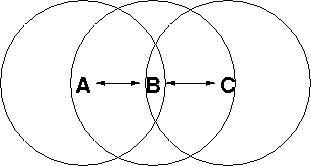
\includegraphics[width=6cm]{hiddenNode-x01.jpg}
    \caption{Illustrating a typical hidden node problem with B being in communication range with A and C.  A is completely out of the communication range of C.}
    \label{fig:hiddenNode}
  \end{center}
\end{figure}

Whenever B broadcasts its OGMs, these messages are received simultaneously by A and C. According to the batman-0.2 algorithm these OGMs are instantly re-broadcasted by node A and node C. Because A and C can not hear each other they have no chance to coordinate their sending using the 802.11 carrier-sense mechanism.

As a consequence (the hidden nodes) A and C will both rebroadcast Bs OGM at almost the same moment and cause a collision at (the exposed node) B. Therefore, node B will miss many of its own OGMs re-broadcasted by its neighboring nodes and will often consider these links as non-bidirectional. Subsequently, node B will ignore OGMs from its neighbors in the neighbor-ranking process due to the failed bidirectional-link check and (if exist) favor an alternative path. This happens, despite having a collusion-free unidirectional connection from B to A and from B to C.

On the other hand, node A (and same for C) is not even aware of that problem. OGMs initiated by A are only heard and re-broadcasted by B and received back by A again. Chances of A and C choosing the same moment for initiating their own OGMs are very rare because every node chooses a random delay for the moment when initiating their own OGMs.

The \emph{--re-brc-delay} switch can be used to configure each node to wait also a random delay before re-broadcasting an OGM received from a neighboring node.
%
This phenomenon can be directly observed as the following debug-information shows:
%
BATMAN running only on B (105.130.0.67) and C (105.131.41.3) :

\begin{small}
\begin{verbatim}
B.A.T.M.A.N. 0.3-exp, MainIF/IP: eth1:bat 105.130.1.67, WindSize: 100, BLT: 2, OGI: 1000, UT: 0d 0h 4m
Originator          viaIF         Router (brc rcvd lseq lvld) [   viaIF RTQ  RQ  TQ].. alternatives...
105.131.41.3    eth1:bat    105.131.41.3 ( 42  42   268    0) [eth1:bat  52  50 100]

B.A.T.M.A.N. 0.3-exp rv641, MainIF/IP: eth1:bat 105.131.41.3, WindSize: 100, BLT: 2, OGI: 1000, UT: 0d 0h 4m
Originator          viaIF         Router (brc rcvd lseq lvld) [   viaIF RTQ  RQ  TQ].. alternatives...
105.130.1.67    eth1:bat    105.130.1.67 ( 62  62   283    1) [eth1:bat  45  89  50]
\end{verbatim}
\end{small}

you can see, that the RTQ (the round-trip-probability), the RQ and the calculated TQ values 
are quite similar from node A and Bs points of view.

when I start batman also on A and wait a while
BATMAN running on A (105.130.30.1), B (105.130.0.67)  and C (105.131.41.3):

\begin{small}
\begin{verbatim}
 
B.A.T.M.A.N. 0.3-exp, MainIF/IP: eth1:bat 105.130.30.1, WindSize: 100, BLT: 2, OGI: 1000, UT: 0d 0h 3m
Originator          viaIF         Router (brc rcvd lseq lvld) [   viaIF RTQ  RQ  TQ].. alternatives...
105.131.41.3    eth1:bat    105.130.1.67 ( 12  12   635    8)
105.130.1.67    eth1:bat    105.130.1.67 ( 60  60   661    0) [eth1:bat  49  90  54]

B.A.T.M.A.N. 0.3-exp, MainIF/IP: eth1:bat 105.130.1.67, WindSize: 100, BLT: 2, OGI: 1000, UT: 0d 0h11m
Originator          viaIF         Router (brc rcvd lseq lvld) [   viaIF RTQ  RQ  TQ].. alternatives...
105.131.41.3    eth1:bat    105.131.41.3 ( 17  17   644    1) [eth1:bat  21  44  47]
105.130.30.1    eth1:bat    105.130.30.1 ( 25  25   217    0) [eth1:bat  27  50  54]

B.A.T.M.A.N. 0.3-exp, MainIF/IP: eth1:bat 105.131.41.3, WindSize: 100, BLT: 2, OGI: 1000, UT: 0d 0h10m
Originator          viaIF         Router (brc rcvd lseq lvld) [   viaIF RTQ  RQ  TQ].. alternatives...
105.130.1.67    eth1:bat    105.130.1.67 ( 56  56   666    0) [eth1:bat  40  85  47]
105.130.30.1    eth1:bat    105.130.1.67 ( 16  16   220    1)

\end{verbatim}
\end{small}

It can be seen that the measured RQ values (at node A and B) did NOT relevantly change (indicating, that the link quality has not really changed). But the measured RTQ value measured at exposed node B (to node A) decreased by almost 50\% due to the collisions. 
Because the TQ value is calculated based on $TQ = RTQ / RQ$ it indicates
a wrong value.
%
A simple test shows that the collision problem could be almost resolved by applying a random delay of up to 15 ms. Using

\begin{small}
\begin{verbatim}
$batmand --window-size 100 --re-brc-delay 15 eth1:bat
\end{verbatim}
\end{small}
%
the debug-level one output now shows:
%
\begin{small}
\begin{verbatim}

B.A.T.M.A.N. 0.3-exp, MainIF/IP: eth1:bat 105.130.30.1, WindSize: 100, BLT: 2, OGI: 1000, UT: 0d 0h 3m
Originator          viaIF         Router (brc rcvd lseq lvld) [   viaIF RTQ  RQ  TQ].. alternatives...
105.131.41.3    eth1:bat    105.130.1.67 ( 24  24   208    0)
105.130.1.67    eth1:bat    105.130.1.67 ( 62  62   197    0) [eth1:bat  53  83  63]

B.A.T.M.A.N. 0.3-exp, MainIF/IP: eth1:bat 105.130.1.67, WindSize: 100, BLT: 2, OGI: 1000, UT: 0d 0h 3m
Originator          viaIF         Router (brc rcvd lseq lvld) [   viaIF RTQ  RQ  TQ].. alternatives...
105.131.41.3    eth1:bat    105.131.41.3 ( 34  34   208    1) [eth1:bat  46  49  93]
105.130.30.1    eth1:bat    105.130.30.1 ( 41  40   195    1) [eth1:bat  45  58  77]

B.A.T.M.A.N. 0.3-exp rv551, MainIF/IP: eth1:bat 105.131.41.3, WindSize: 100, BLT: 2, OGI: 1000, UT: 0d 0h 3m
Originator          viaIF         Router (brc rcvd lseq lvld) [   viaIF RTQ  RQ  TQ].. alternatives...
105.130.1.67    eth1:bat    105.130.1.67 ( 61  61   197    1) [eth1:bat  47  89  52]
105.130.30.1    eth1:bat    105.130.1.67 ( 33  33   195    2)

\end{verbatim}
\end{small}

By enabling the \emph{--re-brc-delay} switch you may also consider to use the accept duplicates switches described below.

It should be mentioned that such a random delay has further side effects.
The most critical is probably that the batman-0.2 algorithm considers only the first OGM (received with a new sequence number) for the neighbor ranking. This way, the batman-0.2 algorithm implements its strong favor for the 
quickest and shortest paths. 

Applying the \emph{--re-brc-delay} parameter, the propagation speed of OGMs is probably more related to the random delay (experienced by each OGM at each intermediate hop) than on the actual number of hops it has passed. You are welcome to continue reading for a deeper discussion about the pros and cons of this side effect.



\subsection{Tradeoff: Long versus short but poor-link paths}

In a wireless multi-hop mesh, there are typically several possible paths between two nodes. 
Assuming the probably most simple setup as illustrated in Figure \ref{fig:longVsPoorHops}, 
each node is in physical communication range of each other. However, with different link qualities.

For packets that need to be delivered from A to C there are two possible paths. The two-hop path from A via B to C and the direct path from A to C.

\begin{figure}[htbp]
  \begin{center}
    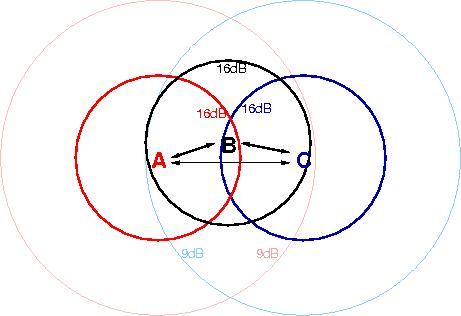
\includegraphics[width=10cm]{longVsPoorHops-x01.jpg}
    \caption{Illustrating the tradeoff between the long two-hop path with good link qualities versus the one-hop path with a poor link quality.}
    \label{fig:longVsPoorHops}
  \end{center}
\end{figure}


Each of the two short links ($A-B$ and $B-C$) has a better link quality than the direct link between A and C. For the first path, each end-to-end packet delivery requires two transmissions. One from A to B and another from B to C.
%
Choosing the direct link, one transmission might be sufficient. This seems to result in a shorter transmission time for the end-to-end packet delivery and being more efficient with the overall bandwidth consumption. But (due to the lower link quality) each transmission is also more prone to errors and therefore might require casual retransmissions. 
%
Probably even more important, the 802.11 MAC layer might choose a less robust but faster data-rate for the packet transmission via the two short links. This would once again decrease the required transmission time and maybe even outperform the transmission via the direct link.
%
According to the receiver performance requirements specified in \cite{ieee80211a} page 31, a signal degradation of 7dB  may result in a data-rate degradation from 18 to 6 MBits/second. In this case, choosing the two-hop path should even pay out when considering the additional transmissions necessary for the extra hop.

The Batman-III algorithm (as implemented in batman-0.2) has a strong favor for short paths -- being rather ignorant about poor links along that path. 
%
This is because:
\begin{itemize}

 \item The end-to-end path established between two batman nodes is the result of the neighbor ranking performed on all intermediate nodes along that path.

 \item Only the first (quickest) OGM received via a specific neighbor is considered for the neighbor ranking. %

 \item All OGMs are broadcasted using an equal and (depending on the WLAN driver) very robust and slow data rate. The link quality in terms of bandwidth is not considered until the link is so lousy that many OGMs get lost.\footnote{Varying and thereby choosing also faster datarates for the emission of OGMs might be a promising approach to tackle this shortcoming.}

 \item Therefore, an OGM received directly from its originator is always quicker than a re-broadcasted OGM received via an intermediate hop. OGMs propagated over a two-hop path are generally quicker that those propagated over a more-than-two-hop path.


\end{itemize}
 
%
Given the scenario illustrated in Figure \ref{fig:longVsPoorHops}, 
whenever an OGM from C is directly received by A, the same OGM is ignored when received via the two-hop path (from C via B to A).
%
Even if all of Cs OGMs that were propagated via the two-hop path C-B-A could be received by A,
 but only 60 \% of Cs OGMs make it via the direct link C - A, the neighbor ranking at node A would still count 60 OGMs for the direct link and only 40 OGMs for the path via neighbor B. Thus, making neighbor C the winner of the neighbor ranking and choosing the direct link for packet delivery from A to C. 
%
Drawing it even more dramatically, the decision could result in favoring a single-hop path with a datarate of 6MBit/s and a packet loss of 40 \% instead of a two-hop path with a per-link datarate of up to 18 MBit/second and no packet loss.



The parameters described in the following can be used to handle this challenge.



\subsubsection{Accept non-quickest OGMs depending on number of additional hops}

%There are two options to give OGMs propagated via the non-shortest path a fair chance in the neighbor ranking.

%\begin{itemize}

% \item Increase the probability for OGMs propagated via the non-shortest path to become the quickest OGM received by a distant node. This could partly be achieved by introducing a random rebroadcast delay as described in Section \ref{sec:re-brc-delay}. However, this approach only helps with competing multi-hop paths where even the shorter path has at least one intermediate hop. If a single-hop path is involved in the neighbor-ranking, no rebroadcating via that path does occur and no random rebroadcast delay is applied.

%\end{itemize}

A straight forward approach to relieve the strong favor for short paths would be to also accept OGMs for the neighbor ranking that propagated via an alternative and non-quickest path. 
%
Thus, also accept OGMs that could be identified as a duplicate (due to the same sequence number and originator IP) of a previously received OGM.
%
But care must been taken to not accept duplicates that travelled a loop.  
%
This could be sorted out by limiting the number of additional hops such a duplicate is allowed to have passed compared to the previously received OGM.
%

Given a similar setup as illustrated in Figure \ref{fig:hiddenNode}, an OGM initiated by node A and rebroadcasted by node B, may subsequently be received and rebroadcasted by node C, and finally be received by node B for a second time. 
%
The OGM has been transmitted from A to B, to C, and back to B again. 
%
In this case, after being received by node B for the first time, the OGM has passed the smallest possible loop with two additional hops.
%
Each additional hop an OGM is propagated along a path, the time to live (TTL) field is decremented by one. 
%
Therefore, each node can easily identify the number of additional hops a non-quickest OGM has passed (compared to the previously received OGM) by comparing contained TTL values.


The limit of additional hops, such duplicate OGMs are allowed to have passed, for being accepted for the neighbor ranking could be configured using the \emph{--dups-ttl} parameter. 
%
Applying a value of 2 would reject every duplicate OGM that passed 2 or more additional hops than any previously received OGM -- ensuring loop-free propagaton of OGMs.
%

\begin{small}
\begin{verbatim}
    Parameter: --dups-ttl <value> 
        Accept non-quickest OGMs to relieve preference for shortest path.
        (< value > - 1) defines how much smaller the TTL of a non-first OGM can be compared to the 
        largest TTL received so fare (with the same originator IP and sequencenumber). 
        default: 0 (disabled), allowed values: 0 <= value <= 10
\end{verbatim}
\end{small}


I recommend to combine the \emph{--dups-ttl} parameter with the \emph{--re-brc-delay} parameter.

Values larger than 2 should not be applied until using also one of the parameters described in the following Section.

\subsubsection{Accept non-quickest OGMs with reduced probability}

%\subsubsection{Accept non-quickest OGMs with probability depending on additional hops}

The problem with looped OGMs is not the OGM itself but the path promoted by that message.
%
The end-to-end path established between two nodes is the result of the neighbor ranking performed on each hop along that path. 
%
If it ever happens that the best-ranking neighbor becomes selected due to looped OGMs, the path established via the selected neighbor causes a routing loop. This should be strictly avoided.
%
On the other hand, from the perspective of each node along that path, this path is only changed if even more recent OGMs are received and accepted via an alternative neighbor, than have been received and accepted via the currently best-ranking neighbor.
%
By ensuring that duplicate (and potentially looped) OGMs are only partially accepted, the number of looped OGMs could never outperform the number of OGMs received via the real best-ranking neighbor.
%

The following two parameters can be used to accept duplicate OGMs only with a reduced probability


\begin{small}
\begin{verbatim}

    Parameter: --dups-rate <value> 
        Accept non-quickest OGMs to relieve preference for shortest path.
        < value > defines the general probability with which non-quickest OGMs are accepted. 
        default: 0 (disabled), allowed values in percent: 0 <= value <= 100


    Parameter: --dups-ttl-degradation <value> 
        Accept non-quickest OGMs to relieve preference for shortest path.
        < value > defines the probability degradation for each additional hop 
        (compared to the OGM arrived via the shortest path) with which non-quickest OGMs are accepted. 
        default: 0 (disabled), allowed values in percent: 0 <= value <=100

\end{verbatim}
\end{small}


%Applying a larger value than 2 is critical as long as all received duplicate OGMs are accepted with a relatively high probability. 

%By accepting only a fraction the received duplicate OGMs, it becomes possible to even consider OGMs that passed more than 2 additional hops for the neighbor ranking. Read more about this in the following section.



\subsection{The impact of asymmetric links}
\label{sec:asymmetric-links}

The phenomenon of an asymmetric link can be observed in every-day life. Given for example the conversation between a Diskjockey and one of his fans as illustrated in Figure \ref{fig:asymmetric-link}. In this scenario the DJ, having his ears covered with booming headphones, is well understood by the fan. But in the other direction, because the DJ is exposed to the noisy music from his headphones, he can not understand anything from his fan. 

\begin{figure}[htbp]
  \begin{center}
    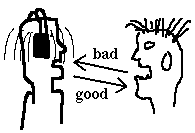
\includegraphics[width=5cm]{KopfoererTyp-x01-selected.png}
    \caption{Illustration of an asymmetric communication channel.}
    \label{fig:asymmetric-link}
  \end{center}
\end{figure}



%
Assigning an overall verdict, one may qualify the quality of the communication channel between the DJ and his fan as \emph{average}. 
%
However, relying on such a verdict would be misleading and inefficient. 
%
From the fans point of view, choosing a redundant but oral transmission technique (for example by speaking loud and slowly, to deliver an important message, will fail. 
%
But if the fan knew about the asymmetry of the link, he may have chosen to write down the message.
%
From the DJs point of view, choosing to speak loud and slowly is simply not necessary.
It is a waste of energy because there is actually no need to speak loudly. And it is inefficient because his message would have been understood even when talking faster.
% 


The impacts of asymmetric links in wireless mesh networks are even more versatile (and probably unknown). The following example shall illustrate this.
%
Considering for example a very simple asymmetric links scenario as given in Figure \ref{fig:asymmetric-path}.


\begin{figure}[htbp]
  \begin{center}
    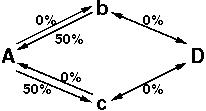
\includegraphics[width=5cm]{asymmetricPathChaos.jpg}
    \caption{Illustration of a simple multi-hop asymmetric-link scenario.}
    \label{fig:asymmetric-path}
  \end{center}
\end{figure}


The figure shows four nodes (A,b,c,D) and four existing links between them $A-b$, $b-D$, $A-c$, and $c-D$. There are two potential end-to-end paths between node A and D, one going via the intermediate node b and another via node c. 
%
The links $b-D$ and $c-D$ are symmetric, perfect links with 0 \% packet loss. 
%
The links $ A - b $ and $ A - c $ are asymmetric links with 0 \% packet loss for the directions $ A \rightarrow b $ and $ c \rightarrow A $, but 50 \% loss for the directions $ b \rightarrow A $ and $ A \rightarrow c $.
%
For the task of delivering a ping request packet from A and D and sending the ping reply back from D to A there are the following four routing options:
\begin{enumerate}
 \item Via $ A \rightarrow b \rightarrow D \rightarrow b \rightarrow A $ with a total round-trip loss of 50 \%.
 \item Via $ A \rightarrow b \rightarrow D \rightarrow c \rightarrow A $ with a total round-trip loss of 0 \%.
 \item Via $ A \rightarrow c \rightarrow D \rightarrow b \rightarrow A $ with a total round-trip loss of 75 \%.
 \item Via $ A \rightarrow c \rightarrow D \rightarrow c \rightarrow A $ with a total round-trip loss of 50 \%.
\end{enumerate}

This example is of course just an naive fallacy compared to the complexity of real-live wireless-mesh networks but it should illustrate the potential efficiency margin that might result from properly or unproperly reflecting asymmetric links.

%One general approach for equipping the routing protocol with appropriate means to efficiently handle such challenges is presented below.


In BATMAN, the link characteristics are differentiated in receive quality (RQ), transmit quality (TQ), and the product of both values $RTQ = RQ * TQ$.
%
%From the DJs point of view (Figure \ref{fig:asymmetric-link}), the RQ of the link to his fan is very bad and the TQ is very good. From the fans point of view its just the other way around. 
%
From node As point of view (Figure \ref{fig:asymmetric-path}), the RQ of the link to neighbor b is 50 \% and the TQ to neighbor b is 100 \%. From node bs point of view its just the other way around. 

The RQ of a specific link is measured by counting the amount of recently received OGMs from the corresponding link neighbor.
%
The RTQ of a specific link is measured by counting the amount of recently received own OGMs, rebroadcasted from the corresponding link neighbor.
%
And the TQ is calculated based on $TQ = RTQ / RQ$.
%
Some further information about link qualities is also given in Section \ref{sec:debug-level-1}.

%In the following further considerations are given dabout the importance of the receive and transmit quality of a link.
%
In the first place, from the senders point of view, the TQ of a given link seems to be more relevant than the corresponding RQ.
%
But the MAC protocol of 802.11 \cite{ieee80211} demands that each unicast transmission from A to B is successfully acknowledged back from B to A. 
%
This demand makes a successfull transmission of the acknowledgment message as important as the unicast-data message itself.
%
On the other hand, the transmission of a MAC acknowledgement is subject to a number of advantages compared to the transmission of a unicast-data message.
 
\begin{itemize}
  \item  The packet size of a MAC acknowledgement is very small and usually very much smaller than the size of the corresponding data packet, leaving a much smaller risk for the Acknowledgment message to collide.

 \item The time slot during which the MAC acknowledgement is to be transmitted has already been reserved by the preceding data packet (with a similar result as the RTS/CTS mechanism could achieve for the data packets).

 \item Last but not least, the MAC acknowledgement are usually transmitted with a much more redundant modulation compared to the modulation used for the preceding data packet. This arms them with some additional resilience against interference and noise.

\end{itemize}


The above discussion provided a rationale for the differentiation of a link quality into its receive and transmit quality. 
%
However, properly weighting the relevance of the RQ and TQ characteristics for an unicast transmission is subject to further experiments. %
Some preliminary but promising weighting factors have been gained from the experiments at the wireless community weekend 2007 in Graz. 
%
The currently proposed parametrization of the batman-experimental implementation is described in Section \ref{sec:proposed-parametrizations}.


%
\subsubsection{Reflecting link qualities with B.A.T.M.A.N}
\label{sec:batman-link-reflection}

The BATMAN-III algorithm establishes routes between nodes based on the number of OGMs  received via a specific neighbor. 
%
This way, the algorithm promotes routes with good receive qualities (from the receiving nodes' point of view). But these routes are then used for sending. 
%
In other words, the OGMs initiated by each node install routing information for DOWN-link traffic which are actually optimized for UP-link traffic. 

Referring to Figure \ref{fig:asymmetric-path}, node A receives 100 \% of the OGMs initiated by D and rebroadcasted via node c. 
%
On the other hand, node A receives only 50 \% of Ds OGMs via node b. 
%
Therefore A would select c as its best-ranking neighbor towards D (obversely D would select b as its best neighbor towards A).

Thereby, the flooding mechanism of BATMAN-III inherently promotes the propagation via links with a good RQ. The reflection of the TQ characteristics could only be achieved indirectly with a very strict bidirectional link check. 
%
But even when applying the strictest possible bi-link-timeout, the total link-quality reflection only sums up to $ TQ * RQ^2 $ per hop, giving the TQ a much smaller influence than the RQ.

BATMAN-IV has the capability to differentiate a link quality into its distinct directions and reflect these characteristics in the path detection algorithm.
%
The idea is, that each node along the propagation path of an OGM expresses negative observations about the link via which an OGM was received by simply reducing the probability with which it accepts and further propagates the received OGM.
%
By intentionally not accepting an OGM for the neighbor ranking, each node has the possibility to counteract on the propagation via specific links and influence the establishment of resulting routes in the mesh.
Only accepted OGMs received via the best-ranking neighbor are reboradcasted.


\subsubsection{Reflecting the link transmit quality (TQ)}

The following parameters exist to configure the acceptance-function when to accept or not to accept a received OGM depending on the TQ to the corresponding link neighbor.

\begin{small}
\begin{verbatim}

       Parameter: --asymmetric-exp <value> : Ignore rcvd OGMs to respect asymmetric-links.
          Ignore with probability TQ^<value>.
          default: 0, allowed exponent values: 0 <= value <= 3

       Parameter: --asymmetric-weight <value> : Ignore rcvd OGMs to respect asymmetric-links.
          default: 0, allowed probability values in percent: 0 <= value <= 100

\end{verbatim}
\end{small}

Regarding the TQ, a received OGM is accepted with probability p, according to following formula:

probability $ p \in [0..1] $

neighbor ranking frame (NBRF) size $s$

link transmit quality $ t \in [0..s] $

asymmetric-exp value $ e \in [0,1,2,3] $

asymmetric-weight value $ w \in [0..100] $

$ p(t) = (w/100) * (t/s)^e $



\subsubsection{Reflecting the link receive quality (RQ)}

As described in Section \ref{sec:batman-link-reflection}, the reflection of the RQ characteristics (along the paths in a mesh) is an inherent characteristic of the flooding algorithm.
%
The previous discussion in Section \ref{sec:asymmetric-links} and \ref{sec:batman-link-reflection} has also indicated that a prevailing reflection of the link-RQs can even be contraproductive for the establishment of performant routes.
 
%
%By accepting received OGMs only with a probability depending on the TQ identified for the incoming link, the flooding mechanism can also reflect the TQ of intermediate links in the promoted paths. 
%
%Actually, the acceptance-function can even be tuned to ignore received OGMs with an  exponential invers ration to the TQ, 
%
%However, the approach of intentionally not accepting a relevant fraction of the received OGMs also has the side effect of decreasing the number of rebroadcasted OGMs with every additional hop. If 
%
Therefore, the question is rather how this inherent behavior can be relieved than how the reflection of the RQ characteristics can be further enforced.
%
Kind of brute-force approach to reduce the influence of a weak RQs is to simply decrease the chance that OGMs get lost. 
%
And one way to achieve that is to simply broadcast OGMs multiple times, increasing the chance that at least one of the multiple times broadcasted OGMs could be received.
%
Besides the obvious disadvantage of an increased protocol-traffic overhead, this approach incorporates also a number of advantages.

\begin{itemize}

 \item By marking the first broadcasted OGM of each sequence number with a dedicated bit, each node can still measure the correct RQ, RTQ, and TQ to their direct neighbors.

 \item By only broadcasting OGMs twice which passed the acceptance-function and which were received via the best-ranking neighbor the amount of additional protocol traffic could be limited.

 \item All previously described mechanisms (for example to reflect the TQ of a link) remain functional.

 \item The impact of the RQs is not fully eliminated. It is still reflected but with a smaller influence.

 \item This approach helps to increase the propagation range (in terms of hops) of the OGMs. 

\end{itemize}

The following parameter exist to configure the flooding mechanism to broadcast the same OGMs even multiple times.
%

\begin{small}
\begin{verbatim}

       --send-clones <value> : (re-)broadcast OGMs with given probability
        /c <value> : attached after an interface name
          to specify an individual re-broadcast probability for this interface.
          default: 100, allowed probability values in percent: 0 <= value <= 300

\end{verbatim}
\end{small}

The parameter takes a probability argument in the range of zero to several hundred.
%
An argument in the range of zero to hundred specifies the probability in \% with which a to-be-propagated OGM is broadcasted once.
%
An argument in of 150 specifies that each to be propagated OGM is broadcasted at least once and with a probability of 50 \% even twice.
%
An argument of 200 specifies that each to-be-broadcasted OGM is broadcasted exactly twice!

The \emph{/c} parameter can be used to configure an individual (re-)broadcast probability for a specific interface. 
This makes particularly sense for wired lan interfaces because such links are usually not showing the huge packet-loss which is typical for wireless links.

%This approach also causes OGMs to dissapear depending on the number of hops and link qualities it has passed.
%
%To counteract on the fast disappearance of OGMs by selectively rebroadcasting accepted OGMs twice.


\section{Customizing the Daemon for Individual Network Requiremets}
%\section{Parameters for Adapting to Fancy Network Environments}
\label{system-adaption}

Batmand-experimental supports a number of parameters to customize the routing daemon for various network environments.

% and the requirements coming along with that.



\subsection{Achieving in-the-field protocol migration}
A typical desire for an already existing mesh network is the possibility to test and compare a new routing protocol before any of the functionality needed by the currently operating protocol is disabled.
%
A straight forward approach to achieve this desire is to execute the new protocol in parallel to the already existing protocol and ensure that none of the two protocols is influencing the other. 
%

The batmand-0.2 and 0.3 implementations already provided all necessary functionality to operate in parallel to OLSR. 
%
The following batmand-experimental parameters can be used to simultaneously run two (or even more) batman versions on the same devices.
Therefore, the following system attributes should be decoupled.
\begin{itemize}

 \item The IP-address ranges (or netmasks) used for each routing protocol should be non-overlapping. Achievable by equipping the already used network interfaces with an additional alias address and a non-overlapping address range.
  
 \item The port numbers (used for transferring protocol data) and the unix-socket (used to obtain runtime-debug informations) must be different. A corresponding parameter is described below.

 \item The routing table used by the different protocols. A corresponding parameter is described below.

 \item The routing-priority rules used for assigning dedicated routing tables to selected address ranges. A corresponding parameter is described below.

 \item Optionally, to simplify monitoring of cpu-load and memory-consumption, the binary name of the daemons should be different. Achievable by renaming the corresponding binary file to an new name before executing it.

\end{itemize}
%
Related examples are also given in Section \ref{sec:howto}.

\subsubsection{Customizing the protocol ports}

By default, batman uses the UDP port 4305 (as assigned by IANA \cite{iana-ports}) for the flooding of OGMs.
This port is referred as batmands base-port.
%
Optionally, the two sequently following port numbers are used for gateway connectivity and visualization.
%
The port number (base-port + 1) is used for tunneling packets between internet-gateway nodes and client nodes. 
The port number (base-port + 2) is used for sending visualization data to a dedicated visualization server.
The base-port can be configured with the following parameter.


\begin{small} \begin{verbatim}
       --base-port <value> : set base udp port used by batmand.
          <value> for OGMs, <value+1> for GW tunnels, <value+2> for visualization server.
          default: 4305, allowed values: 1025 <= value <= 60000
\end{verbatim} \end{small}

Whenever applying the \emph{--base-port} parameter during the execution of the main daemon, this parameter must be applied again and with the same value for obtaining the correct debug informations. A simple example is given below.

\begin{small} \begin{verbatim}
root@ng1e:~# ln -s /usr/sbin/batmand /usr/sbin/bmxd
root@ng1e:~# bmxd --base-port 24305 --rt-table-offset 77 --prio-rules-offset 26600 ath0:bmx
WARNING: You are using the experimental batman branch!
Long option: base-port with argument: 24305
Long option: rt-table-offset with argument: 77
Long option: prio-rules-offset with argument: 26600
Using interface ath0:bmx with address 103.130.30.201 and broadcast address 103.255.255.255
root@ng1e:~#
root@ng1e:~# bmxd --base-port 24305 -c -d 1 -b
WARNING: You are using the experimental batman branch!
Long option: base-port with argument: 24305
B.A.T.M.A.N. 0.3-exp rv687, MainIF/IP: ath0:bmx 103.130.30.201, WindSize: 128, BLT: 2, OGI: 1000, UT: 0d 0h 2m
Originator           viaIF         Router (brc rcvd lseq lvld) [    viaIF RTQ  RQ  TQ].. alternatives...
103.130.30.202   ath0:bmx  103.130.30.202 ( 26  26    95    0) [ ath0:bmx  26  95  35]
root@ng1e:~#

\end{verbatim} \end{small}

\subsubsection{Customizing the used routing table and priority rules}

The following switches can be used to change the default routing tables and the priority rules. 

\begin{small} \begin{verbatim}
       --rt-table-offset <value> : set base routing table used by batmand.
          <value> for HNA routes, <value+1> for host routes, <value+2> for GW routes.
          default: 65, allowed values: 2 <= value <= 250

       --prio-rules-offset <value> : set base ip-rules priority used by batmand.
          default: 6600, allowed values: 3 <= value <= 32765
\end{verbatim} \end{small}

\subsection{Reconfiguring network integration}

\begin{small} \begin{verbatim}

       --no-unreachable-rule : does not set the unreachable rule for host routes.

       --no-prio-rules : does not set the default priority rules.

       --no-throw-rules : does not set the default throw rules.

       --resist-blocked-send : lets daemon survive if firewall blocks outgoing OGMs.

\end{verbatim} \end{small}

\subsection{Hiding local topology information beyond the neighborhood}

Nodes may alter (i.e. reduce) the default TTL of their own OGMs to limit the number of hops that these OGMs are propagated through the mesh. 
This can be done for all OGMS or just for OGMs propagating the existence of particular interfaces. 
This does not affect the routing between other nodes in the mesh, but may be used to limit the range of presence (existence) of individual nodes. 
For example, a node with three interfaces may be configured to send OGMs with a high TTL only for the first interface and a TTL of one for OGMs representing the second and third interface. 
%
This way, the node is still reachable via the IP of it's first interface. 
But it does not burden the nodes beyond its neighbor horizon with the efforts of maintaining and re-broadcasting OGMs from it's second and third interface.

One side effect of the one-TTL OGMs is that traffic generated on these nodes may leave the node with the source address
of such a secondary interface. 
%which is not known beyond the neighbor horizon of the node.
%
This has the consequence that non-neighboring nodes could not reply to this source address, simply because the OGMs for this source address have never been propagated that fare.
A Solution to counter the above problem is to automatically make an HNA announcement for all "hidden interfaces". 
%Because of the policy-routing (enabled since 0.3) this approach could easily be integration in the current code. 
This behavior is can be enabled using the interface-specific \emph{/a} switch. 

The following parameters can be used to reduce the TTL of OGMs representing specific interfaces.

\begin{small} \begin{verbatim}
       --t <value> : change default TTL of originator packets.
        /t <value> : attached after an interface name
          to change the TTL only for the OGMs representing a specific interface
          default: 50, allowed values: 1 <= value <= 63

        /i : attached after an interface name
          to broadcast the OGMs representing this interface only via this interface,
          also reduces the TTL for OGMs representing this interface to 1.

        /a : attached after an interface name
          to add the IP address of this interface to the HNA list. Also
          reduces the TTL for OGMs representing this interface to 1 and
          broadcasts the OGMs representing this interface only via this interface
\end{verbatim} \end{small}


Especially for (back-bone) nodes, which are not supposed to generate pay-load traffic itself and which were only installed to improve the connectivity and coverage of the mesh by relaying other nodes traffic, the possibility of using a small TTL for all their OGMs comes with the following advantages.
Firstly, the topology and even the existence of the back-bone nodes could be completely hidden beyond their local neighbor horizon and secondly, the number of back-bone nodes (and resulting coverage) can be increased to any size with virtually no side affects to the overall traffic and processing cost.


\subsection{Miscellaneous}


\begin{small} \begin{verbatim}

       --no-unresp-gw-check : disables the unresponsive-GW check.

       --gw-change-hysteresis <vlue>: Use hysteresis for fast-switch gw connections (-r 3).
          <value> for number additional rcvd OGMs before changing to more stable GW.
          default: 1, allowed values: 1 <= value <= 65

\end{verbatim} \end{small}





%%%%%%%%%%%%%%%%%%%%%%%%%%%%%%%%%%%%%%%%%%%%%%%%%%%%%%%%%%%%%%%%%
%%%%%%%%%%%%%%%%%%%%%%%%%%%%%%%%%%%%%%%%%%%%%%%%%%%%%%%%%%%%%%%%%
%%%%%%%%%%%%%%%%%%%%%%%%%%%%%%%%%%%%%%%%%%%%%%%%%%%%%%%%%%%%%%%%%

\section{Proposed Parametrization Sets}
\label{sec:proposed-parametrizations}

Batmand-experimental implements a number of proconfigured parametrization sets.
These parametrization sets have been gained from (subjectively) successfull experiments and deployments.
The parameters applied by a specific set can be overwitten by subsequent parameters.

The parametrization applied by a specific set is always revealed during startup sequence.

\subsection{The --bmx-defaults switch}

The \emph{--bmx-defaults} switch is supposed to always enable the latest and most promising mechanisms that
are available in the current implementation. 
Therefore, configured parameters and values will change with future code versions.

When writing this document, this directive assigned the same parameters as described in Section \ref{sec:graz-2007-switch}.

See the daemons initialization printout to obtain information about the performed parametrization.


\subsection{The --graz-2007 switch}

This switch reflects the experience gained at the wireless community weekend in Graz 2007.
As described, related parametrizations can be obtained from the daemons initialization printout. 

\begin{small} \begin{verbatim}
root@ng2e:~# batmand --bmx-default ath0:bat eth0.0:bat
WARNING: You are using the experimental batman branch!
Applying graz-2007 !
This parametrization expects the first given interface argument to be a wireless interface !
Parametrization based on experience gained from the Wireless Community Weekend in Graz 2007!
Short option: o with argument: 1500
Long option: bi-link-timeout with argument: 20
Long option: window-size with argument: 100
Long option: gw-change-hysteresis with argument: 2
Long option: dups-ttl with argument: 2
Long option: dups-rate with argument: 100
Long option: dups-ttl-degradation with argument: 2
Long option: send-clones with argument: 200
Long option: asymmetric-weight with argument: 100
Long option: asymmetric-exp with argument: 1
Long option: re-brc-delay with argument: 35
Using interface ath0:bat with address 10.10.0.2 and broadcast address 10.10.255.255
Using interface eth0.0:bat with address 10.10.1.2 and broadcast address 10.10.255.255
Interface eth0.0:bat specific option: /a
Interface eth0.0:bat specific option: /i
Interface eth0.0:bat specific option: /t 1
Interface eth0.0:bat specific option: /c 100
root@ng2e:~#
\end{verbatim} \end{small}



%\subsection{The fast-handover switch}

%%%%%%%%%%%%%%%%%%%%%%%%%%%%%%%%%%%%%%%%%%%%%%%%%%%%%%%%%%%%%%%%%
%%%%%%%%%%%%%%%%%%%%%%%%%%%%%%%%%%%%%%%%%%%%%%%%%%%%%%%%%%%%%%%%%
%%%%%%%%%%%%%%%%%%%%%%%%%%%%%%%%%%%%%%%%%%%%%%%%%%%%%%%%%%%%%%%%%


\section{Short Tutorial}
\label{sec:howto}

%\subsection{Setting up a basic testbed}
\label{sec:howto-basics}

This Section provides a brief summary how to setup a simple three-nodes mesh network using the batmand-experimental routing daemon. 
%
The tutorial describes all necessary (and some optionally) steps in an enumerated order. 
%
The following description is working towards a setup as illustrated in Figure \ref{fig:howto-setup}.
Starting with two and working towards three nodes, each having one wireless lan and one optionally wired lan interface.
\begin{enumerate}

\item The following libraries and kernel functionality must be available:

\begin{itemize}
 \item wireless extensions, iwconfig, ifconfig, TUN and IP\_ADVANCED\_ROUTER support in the kernel and the iproute2 tool. Usually this is already installed on your system. You can simply test this by executing the ip or iwconfig binaries or grep for the loaded tun module as done in the following example:
%
\begin{small} \begin{verbatim}
root@ng1e:~# ip rule
0:      from all lookup local
32766:  from all lookup main
32767:  from all lookup default

root@ng1e:~#root@ng1e:~# iwconfig
lo        no wireless extensions.

eth0      no wireless extensions.

ath0      IEEE 802.11g  ESSID:"batman-test"  Nickname:""
          Mode:Ad-Hoc  Frequency:2.412 GHz  Cell: 02:CA:FF:EE:BA:BE
          Bit Rate:0 kb/s   Tx-Power=15 dBm   Sensitivity=1/1
          Retry:off   RTS thr:off   Fragment thr:off
          Encryption key:off
          Power Management:off
          Link Quality=60/70  Signal level=-36 dBm  Noise level=-96 dBm
          Rx invalid nwid:547  Rx invalid crypt:0  Rx invalid frag:0
          Tx excessive retries:0  Invalid misc:0   Missed beacon:0

root@ng1e:~# lsmod | grep tun
tun                     6496  0

root@ng1e:~#
\end{verbatim} \end{small} 

\item On a mipsel-openWrt-based system like freifunk libpthread, tun support, iwconfig, and the batmand-experimental (installed at /usr/sbin/batmand) binaries can be installed with:
%
\begin{tiny}  \begin{verbatim}
root@ng1e:~# ipkg install kmod-tun libpthread freifunk-openwrt-compat
root@ng1e:~# ipkg install http://downloads.open-mesh.net/batman/development/wrt-freifunk/batmand-exp_0.3-exp-current_mipsel-wr-elf-32-lsb-dynamic.ipk
root@ng1e:~# modprobe kmod-tun
\end{verbatim} \end{tiny} 

\item For a i386-based system pre-compiled binaries can be downloaded and installed at /usr/sbin/batmand with:
\begin{tiny}  \begin{verbatim}
root@ng1e:~# wget http://downloads.open-mesh.net/batman/development/i386/batmand-exp_0.3-exp-current_i386-gc-elf-32-lsb-static.tgz
root@ng1e:~# tar xvzf batmand-exp_0.3-exp-current_i386-gc-elf-32-lsb-static.tgz
root@ng1e:~# mv batmand-exp_0.3-exp-*_i386-gc-elf-32-lsb-static /usr/sbin/batmand
\end{verbatim} \end{tiny} 

\item If you have a firewall it must be opened respectively. The easiest way to do so is to accept all IP packets with the example netmask of 10.10.0.0/16:

\begin{small} \begin{verbatim}
root@ng1e:~# iptables -I INPUT   1  -s 10.10.0.0/16 -j ACCEPT
root@ng1e:~# iptables -I INPUT   1  -d 10.10.0.0/16 -j ACCEPT
root@ng1e:~# iptables -I OUTPUT  1  -s 10.10.0.0/16 -j ACCEPT
root@ng1e:~# iptables -I OUTPUT  1  -d 10.10.0.0/16 -j ACCEPT
root@ng1e:~# iptables -I FORWARD 1  -s 10.10.0.0/16 -j ACCEPT
root@ng1e:~# iptables -I FORWARD 1  -d 10.10.0.0/16 -j ACCEPT
\end{verbatim} \end{small}

\end{itemize}

\item After having all the necessary tools available, the involved network interfaces on each node must be configured. 
%
Starting with only two nodes, each running batmand on one wireless interface. 
%
Assuming your wireless interfaces are labelled \verb wlan0. The wireless parameters of all nodes must be configured with the same essid (e.g. batman-test), channel (e.g 10), and mode (ad-hoc). Using iwconfig 
\begin{small} \begin{verbatim}
root@ng1e:~# iwconfig ath0 mode ad-hoc essid batman-test channel 1
\end{verbatim} \end{small} 

We are using a 10.10.0.0/16 network where all wireless interfaces shall become a 10.10.0.x address and the optionally wired interfaces get a 10.10.1.x address. 
%
Using alias interfaces, node A is configured like:
\begin{small} \begin{verbatim}
root@ng1e:~# ifconfig ath0:bat 10.10.0.1 netmask 255.255.0.0 broadcast 10.10.255.255
\end{verbatim} \end{small}
%
The wireless interface on node B is configured using:
\begin{small} \begin{verbatim}
root@ng1e:~# ifconfig wlan0:bat 10.10.0.2 netmask 255.255.0.0 broadcast 10.10.255.255
\end{verbatim} \end{small}

Finally it should be possible to do a first connectivity test. 
%
Because the wlan interfaces of both nodes are in communication range of each other (I am assuming that the testbed has been setup in the same room or so) and have the same netmask they should be link local. A successfull ping on node A to node B should verify this.
\begin{small} \begin{verbatim}
root@ng1e:~# ping 10.10.0.2
PING 10.10.0.2 (10.10.0.2): 56 data bytes
64 bytes from 10.10.0.2: icmp_seq=0 ttl=64 time=5.1 ms
64 bytes from 10.10.0.2: icmp_seq=1 ttl=64 time=2.2 ms

--- 10.10.0.2 ping statistics ---
2 packets transmitted, 2 packets received, 0% packet loss
round-trip min/avg/max = 2.2/3.6/5.1 ms
root@ng1e:~# 
\end{verbatim} \end{small}

\item Now everything is ready to start batmand. Simply execute the daemon on both nodes with the name of the configured wlan interface as its only parameter. The output on node B will show somethink like:

\begin{small} \begin{verbatim}
root@ng2e:~# batmand ath0:bat
WARNING: You are using the experimental batman branch!
Using interface ath0:bat with address 10.10.0.2 and broadcast address 10.10.255.255
root@ng2e:~#
\end{verbatim} \end{small}

\item After executing the binaries they just fork to the background and the prompt is available again. 
Launching the \emph{ps} command should show the process running in the background (The reason for seeing the process several times is a sideeffect of the threaded processing of the daemon. It can be ignored). 
The first feedback from the routing daemon may be obtained with the debug-level-one output. 
Therefore execute batmand a second time with the arguments \emph{ -c -d 1 }. 
The argument \emph{-c} tells batmand to connect to a running batman daemon. 
The argument \emph{-d 1} tells the batmand to printout debug-level-one informations and 
\emph{-b} tells batmand to provide this information only once. 
If \emph{-b} is omitted, the debug information will be updated every second until the process is terminated using \emph{ctrl-c}.
Try this afterwards.

\begin{small} \begin{verbatim}
root@ng2e:~# batmand -c -d 1 -b
WARNING: You are using the experimental batman branch!
B.A.T.M.A.N. 0.3-exp rv686, MainIF/IP: ath0:bat 10.10.0.2, WindSize: 128, BLT: 2, OGI: 1000, UT: 0d 0h12m
Originator           viaIF         Router (brc rcvd lseq lvld) [    viaIF RTQ  RQ  TQ].. alternatives...
10.10.0.1        ath0:bat       10.10.0.1 (112 112   785    0) [ ath0:bat 112 127 112]
root@ng2e:~#
\end{verbatim} \end{small}

The debug-level-one output reveals a number of informations. The first line shows the batmand branch, the revision, the label and ip address of the first interface parameter, the window size, the bidirectional link timeout, the originator interval and the amount of time passed since this process was started. 

The next line shows the headline of a table. 
In our case the table has only one entry which indicates that node B has learned about the existence of node A.
The line starts with the IP of the other batman node, followed by the interface used for routing towards that node, and the best-ranking neighbor used as gateway towards that node. In this case the best-ranking neighbor towards node A is already node A.
For more informations about the informations revealed with debug-level-one see Section \ref{sec:debug-level-1}.

\item You can use the iproute2 tool to investigate the changes batmand has caused to the networking stack.

\begin{small} \begin{verbatim}
root@ng2e:~# ip rule
0:      from all lookup local
6600:   from all to 10.10.0.0/16 lookup 66
6699:   from all lookup 65
6700:   from all to 10.10.0.0/16 lookup 67
32766:  from all lookup main
32767:  from all lookup default
root@ng2e:~# ip route list table 65
root@ng2e:~# ip route list table 66
10.10.0.1 dev ath0  proto static  scope link  src 10.10.0.2
root@ng2e:~# ip route list table 67
unreachable default  proto static
root@ng2e:~#
\end{verbatim} \end{small}

Comparing to the first time we started the \emph{ip rule} command (when we checked if the iproute2 tool is properly working), the output of this command shows three new lines. 
These new lines are priority rules. 
They are telling the networking stack to look out for routes towards the 10.10.0.0/16 address space in dedicated ruting tables -- namely table 66 and 67. 
Using the command \emph{ip route list table 66} the content of table 66 can be further investigated. 

The \emph{ip rule} command also revealed that the ip stack will look out for all kinds of target-ip addresses in table 65. This table is used for network announcements as we will see soon.

\item The batman daemons can be killed with \emph{killall batmand}. Afterwards all configurations made to the networking stack should be cleaned up again.

\item Next, we introduce one additional link and involve the node C into the mesh. 
Therefore we configure the lan interfaces on the three nodes and plug an ethernet cable between the lan interface of node B and node C. 
Assuming the lan interfaces are labelled eth0, one of the following must be executed on each corresponding node.

\begin{small} \begin{verbatim}
root@ng1e:~# ifconfig eth0:bat 10.10.1.1 netmask 255.255.0.0 broadcast 10.10.255.255

root@ng2e:~# ifconfig eth0:bat 10.10.1.2 netmask 255.255.0.0 broadcast 10.10.255.255

root@ng3e:~# ifconfig eth0:bat 10.10.1.3 netmask 255.255.0.0 broadcast 10.10.255.255
\end{verbatim} \end{small}

Be aware, that now node A and B have two interfaces configured for batmand (the lan and the wlan interface) but node C has only the lan interface configured.

\item This time the batman daemon on node A and B must be executed with two trailing interface arguments (\emph{ath0:bat eth0:bat}) where on node C only the single lan interface argument \emph{eth0:bat} must be applied. 
On node B the procedure will look like this:

\begin{small} \begin{verbatim}
root@ng2e:~# batmand ath0:bat eth0:bat
WARNING: You are using the experimental batman branch!
Using interface ath0:bat with address 10.10.0.2 and broadcast address 10.10.255.255
Using interface eth0:bat with address 10.10.1.2 and broadcast address 10.10.255.255

root@ng2e:~# batmand -c -d 1 -b
WARNING: You are using the experimental batman branch!
B.A.T.M.A.N. 0.3-exp rv686, MainIF/IP: ath0:bat 10.10.0.2, WindSize: 128, BLT: 2, OGI: 1000, UT: 0d 0h52m
Originator           viaIF         Router (brc rcvd lseq lvld) [    viaIF RTQ  RQ  TQ].. alternatives...
10.10.1.3        eth0:bat       10.10.1.3 ( 70  70   178    0) [ eth0:bat  70  70 128]
10.10.0.1        ath0:bat       10.10.0.1 (100 100  3044   45) [ ath0:bat  83 128  83]
10.10.1.1        ath0:bat       10.10.0.1 ( 99  99  3041   45)
root@ng2e:~#  
\end{verbatim} \end{small}

The debug-level-one output on node B now shows also the outgoing interface and best-ranking neighbor towards lan interface of node A and the wlan interface of node C.
The debug-level-one output on node C should show:
\begin{small} \begin{verbatim}
root@ng3e:~# batmand -c -d 1 -b
WARNING: You are using the experimental batman branch!
B.A.T.M.A.N. 0.3-exp rv686, MainIF/IP: eth0:bat 10.10.1.3, WindSize: 128, BLT: 2, OGI: 1000, UT: 0d 0h10m
Originator           viaIF         Router (brc rcvd lseq lvld) [    viaIF RTQ  RQ  TQ].. alternatives...
10.10.0.2        eth0:bat       10.10.1.2 (128 128  3581    0)
10.10.1.2        eth0:bat       10.10.1.2 (128 128  3583    0) [ eth0:bat 128 128 128]
10.10.0.1        eth0:bat       10.10.1.2 ( 24  24  3465   52)
10.10.1.1        eth0:bat       10.10.1.2 ( 24  24  3461   52)
root@ng3e:~#
\end{verbatim} \end{small}

\item So fare (despite the different looking debug-level-one output) everything behaved just with like with batmand-0.2
%
Now it is time to make the first experiments with some batmand-experimental concepts.
Therefore we once again \emph{killall batmand} processes and relaunch them with the \emph{--bmx-defaults} argument as shown for node A:

\begin{small} \begin{verbatim}
root@ng1e:~# batmand --bmx-defaults ath0:bat eth0:bat
WARNING: You are using the experimental batman branch!
Long option: bmx-defaults
Short option: o with argument: 1500
Long option: bi-link-timeout with argument: 20
Long option: window-size with argument: 100
Long option: gw-change-hysteresis with argument: 2
Long option: dups-ttl with argument: 2
Long option: dups-rate with argument: 100
Long option: dups-ttl-degradation with argument: 2
Long option: send-clones with argument: 200
Long option: asymmetric-weight with argument: 100
Long option: asymmetric-exp with argument: 1
Long option: re-brc-delay with argument: 35
Using interface ath0:bat with address 10.10.0.1 and broadcast address 10.10.255.255
Using interface eth0:bat with address 10.10.1.1 and broadcast address 10.10.255.255
Interface eth0:bat specific option: /a
Interface eth0:bat specific option: /i
Interface eth0:bat specific option: /t 1
Interface eth0:bat specific option: /c 100
root@ng1e:~#
root@ng1e:~# echo dont forget to start batmand --bmx-defaults... also on the other nodes before continueing
dont forget to start batmand --bmx-defaults... also on the other nodes before continueing
root@ng1e:~#
root@ng1e:~# batmand -c -d 1 -b
WARNING: You are using the experimental batman branch!
B.A.T.M.A.N. 0.3-exp rv686, MainIF/IP: ath0:bat 10.10.0.1, WindSize: 100, BLT: 20, OGI: 1500, UT: 0d 0h 3m
Originator           viaIF         Router (brc rcvd lseq lvld) [    viaIF RTQ  RQ  TQ].. alternatives...
10.10.0.2        ath0:bat       10.10.0.2 ( 28  69   169    1) [ ath0:bat  63 100  63]
10.10.1.3        ath0:bat       10.10.0.2 ( 25  69   195    0)
root@ng1e:~# 

\end{verbatim} \end{small}

to be continued...


\end{enumerate}



%\subsection{Setting up an internet-gateway node}
\label{sec:howto-gw}

%\subsection{Setting up an internet-client node}
\label{sec:howto-client}



%%%%%%%%%%%%%%%%%%%%%%%%%%%%%%%%%%%%%%%%%%%%%%%%%%%%%%%%%%%%%%%%%
%%%%%%%%%%%%%%%%%%%%%%%%%%%%%%%%%%%%%%%%%%%%%%%%%%%%%%%%%%%%%%%%%
%%%%%%%%%%%%%%%%%%%%%%%%%%%%%%%%%%%%%%%%%%%%%%%%%%%%%%%%%%%%%%%%%
\section {Acknowledgments}
\label{sec:acks}

The B.A.T.M.A.N. mesh routing protocol is currently developed by:

Andreas Langer (a.langer-at-q-dsl.de)

Axel Neumann (axel-at-open-mesh.net)

Corinna 'Elektra' Aichele (onelektra-at-gmx.net)

Ludger Schmudde (lui-at-schmudde.com)

Marek Lindner (lindner\_marek-at-yahoo.de)

Simon Wunderlich (siwu-at-hrz.tu-chemnitz.de)

Stefan Sperling (stsp-at-stsp.in-berlin.de)

Wesley Tsai (wesleyboy-at-gmail.com)









%\bibliography{biblio}


\begin{thebibliography}{1}

\bibitem{wesley-batmand-howto} 
{Wesley Tsai},
{\it B.A.T.M.A.N Daemon HowTo}, {August 8, 2007},\\
{http://open-mesh.net/batman/doc/batmand\_howto.pdf}

\bibitem{wesley-batmand-manpage} 
{Wesley Tsai},
{\it BATMAND manpage},\\
{http://downloads.open-mesh.net/batman/development/sources/batmand\_0.3-beta-current\_sources/man/batmand.8.html}

\bibitem{svn-batmand-install} 
{batmand subversion repository},\\
{https://dev.open-mesh.net/svn/batman/trunk/batman/INSTALL}

\bibitem{bmx-source-url}
{batmand-experimental download URL},\\
{http://downloads.open-mesh.net/batman/development/sources/batmand-exp\_0.3-exp-current\_sources.tgz}


\bibitem{batman-status-report} 
{Axel Neumann, Corinna 'Elektra' Aichele, Marek Lindner},
{\it B.A.T.M.A.N Status Report}, {June 28, 2007},
{http://open-mesh.net/batman/doc/batman-status.pdf}

\bibitem{batman-specification-wiki} 
{\it B.A.T.M.A.N Protocol Specification}, {online wiki},\\
{http://open-mesh.net/batman/doc/specification}


\bibitem{ieee80211}
	{\it IEEE 802.11-1999, 1999 Edition (R2003): "Wireless LAN Medium
	Access Control (MAC) and Physical Layer (PHY) Specifications},
%	{\it IEEE 802.11 },
  {June, 12 2003},	
	http://standards.ieee.org/getieee802/802.11.html

\bibitem{ieee80211a}
	{\it IEEE 802.11a-1999(R2003): "Wireless LAN Medium Access Control (MAC) and Physical Layer (PHY) Specifications},
	{\it High-speed Physical Layer in the 5GHz Band },
  {June, 12 2003},	
	http://standards.ieee.org/getieee802/download/802.11a-1999.pdf

\end{thebibliography}

\section*{Licence}

Copyright (C) 2007 Axel Neumann (axel-at-open-mesh.net) \\
Last updated \today\\
Licensed under the Creative Commons BY-NC-SA-2.0 \\
http://creativecommons.org/licenses/by-nc-sa/2.0/

\end {document}

